\documentclass[12pt,a4paper]{article}
% Russian support
\usepackage[T2A]{fontenc}
\usepackage[utf8]{inputenc}
\usepackage[russian]{babel}
% Math, URL, layout
\usepackage{amsmath,amssymb,amsthm}
\usepackage{geometry}
\usepackage{hyperref}
\usepackage{microtype}
\usepackage{setspace}
\usepackage{caption}
\usepackage{graphicx}
\geometry{
  left=25mm,
  right=25mm,
  top=25mm,
  bottom=25mm
}
\hypersetup{
  colorlinks=true,
  linkcolor=black,
  urlcolor=blue,
  pdfauthor={Тишковец Сергей},
  pdftitle={Отчёт по лабораторной работе №1 — Интервальный анализ}
}
\begin{document}
\selectlanguage{russian}
\begin{titlepage}
  \begin{center}
    {Санкт-Петербургский политехнический университет Петра Великого\\
    Институт прикладной математики и механики\\[0.5em]
    \textbf{Высшая школа прикладной математики и вычислительной физики}}
   
    \vfill
   
    {\LARGE\bfseries Отчёт по курсовой работе\\ Часть №1\par}
    \vspace{1em}
    {\Large по дисциплине\\[0.3em] {\bfseries «Проект по математической статистике»}}
   
    \vfill
   
    \begin{flushright}
        Выполнил\\
        студент гр. 5030102/20202: Тишковец Сергей
    \end{flushright}
   
   
    \begin{flushright}
        Проверил\\
        Преподаватель: Заяц Олег Иванович
    \end{flushright}
   
    \vfill
    Санкт-Петербург\\
    2026
  \end{center}
\end{titlepage}
\setcounter{page}{2}
\newpage

\section*{Вычисление ОИСКО: Равномерное распределение и колокольное ядро}

Задана плотность равномерного распределения с нулевым математическим ожиданием и единичной дисперсией:

\[
f_0(x) = 
\begin{cases}
\dfrac{1}{2\sqrt{3}}, & |x| \le \sqrt{3}, \\
0, & |x| > \sqrt{3}.
\end{cases}
\]

Задана плотность колокольного ядра:
$$K(x) = \frac{1}{\sqrt{2\pi}} e^{-\frac{x^2}{2}}$$

Найдем их характеристические функции:
$$E_0(z) = \int_{-\sqrt{3}}^{\sqrt{3}} \frac{1}{2\sqrt{3}} e^{izx} dx = \frac{e^{iz\sqrt{3}} - e^{-iz\sqrt{3}}}{2i\sqrt{3}z} = \frac{\sin(z\sqrt{3})}{z\sqrt{3}}$$
$$E_K(z) = \int_{-\infty}^{\infty} \frac{1}{\sqrt{2\pi}} e^{-\frac{x^2}{2}} e^{izx} dx = e^{-\frac{z^2}{2}}$$

Относительное интегральное среднеквадратическое отклонение (ОИСКО) вычисляется по формуле:
$$\bar{\delta}_n(\xi) = 1 + \frac{I_1}{n\xi I_4} + \left(1 - \frac{1}{n}\right)\frac{I_2(\xi)}{I_4} - 2\frac{I_3(\xi)}{I_4}$$

Вычислим необходимые интегралы.

\subsection*{1. Вычисление $I_1$ и $I_4$}
$$I_1 = \int_{-\infty}^{\infty} |E_K(z)|^2 dz = \int_{-\infty}^{\infty} e^{-z^2} dz = \sqrt{\pi}$$

$$I_4 = \int_{-\infty}^{\infty} |E_0(z)|^2 dz = \int_{-\infty}^{\infty} \frac{\sin^2(z\sqrt{3})}{3z^2} dz$$
Используя табличный интеграл $\int_{-\infty}^{\infty} \frac{\sin^2(ax)}{x^2} dx = a\pi$, получаем:
$$I_4 = \frac{1}{3} \cdot \sqrt{3}\pi = \frac{\pi}{\sqrt{3}}$$

\subsection*{2. Вычисление $I_2(\xi)$}
$$I_2(\xi) = \int_{-\infty}^{\infty} |E_0(z)|^2 |E_K(\xi z)|^2 dz = \frac{2}{3} \int_{0}^{\infty} \frac{\sin^2(z\sqrt{3})}{z^2} e^{-\xi^2 z^2} dz$$
Рассмотрим параметрический интеграл $J(a, b) = \int_{0}^{\infty} \frac{\sin^2(ax)}{x^2} e^{-bx^2} dx$. Дифференцируя по $a$ и используя свойства интеграла вероятностей, можно показать, что:
$$J(a,b) = \frac{\pi a}{2} \text{erf}\left(\frac{a}{\sqrt{b}}\right) + \frac{\sqrt{\pi b}}{2} \left(e^{-\frac{a^2}{b}} - 1\right)$$

где функция ошибок определяется как
\[
\text{erf}(x) = \frac{2}{\sqrt{\pi}} \int_{0}^{x} e^{-t^2} \, dt.
\]

Подставим $a = \sqrt{3}$ и $b = \xi^2$:
$$J(\sqrt{3}, \xi^2) = \frac{\pi \sqrt{3}}{2} \text{erf}\left(\frac{\sqrt{3}}{\xi}\right) + \frac{\xi\sqrt{\pi}}{2} \left(e^{-\frac{3}{\xi^2}} - 1\right)$$
Тогда интеграл $I_2(\xi)$ равен:
$$I_2(\xi) = \frac{2}{3} J(\sqrt{3}, \xi^2) = \frac{\pi}{\sqrt{3}} \text{erf}\left(\frac{\sqrt{3}}{\xi}\right) + \frac{\xi\sqrt{\pi}}{3} \left(e^{-\frac{3}{\xi^2}} - 1\right)$$

\subsection*{3. Вычисление $I_3(\xi)$}
$$I_3(\xi) = \int_{-\infty}^{\infty} |E_0(z)|^2 E_K(\xi z) dz = \frac{2}{3} \int_{0}^{\infty} \frac{\sin^2(z\sqrt{3})}{z^2} e^{-\frac{\xi^2}{2} z^2} dz$$
Заметим, что это тот же интеграл $I_2$, но с заменой параметра $\xi$ на $\frac{\xi}{\sqrt{2}}$. Следовательно:
$$I_3(\xi) = I_2\left(\frac{\xi}{\sqrt{2}}\right) = \frac{\pi}{\sqrt{3}} \text{erf}\left(\frac{\sqrt{6}}{\xi}\right) + \frac{\xi\sqrt{\pi}}{3\sqrt{2}} \left(e^{-\frac{6}{\xi^2}} - 1\right)$$

\subsection*{Итоговая формула ОИСКО}
Подставляя полученные интегралы в исходную формулу, получаем финальное точное аналитическое выражение для ОИСКО:
$$\bar{\delta}_n(\xi) = 1 + \frac{\sqrt{3}}{\sqrt{\pi}n\xi} + \left(1 - \frac{1}{n}\right) \frac{\sqrt{3}}{\pi} I_2(\xi) - \frac{2\sqrt{3}}{\pi} I_3(\xi)$$
где $I_2(\xi)$ и $I_3(\xi)$ определены выше.

\section*{Построение графиков}

Для визуального анализа поведения ОИСКО были построены следующие графики.
\newpage
\subsection*{График 1. Зависимость ОИСКО \(\bar{\delta}_n(\xi)\) от параметра \(\xi\)}

\begin{figure}[ht!]
    \centering
    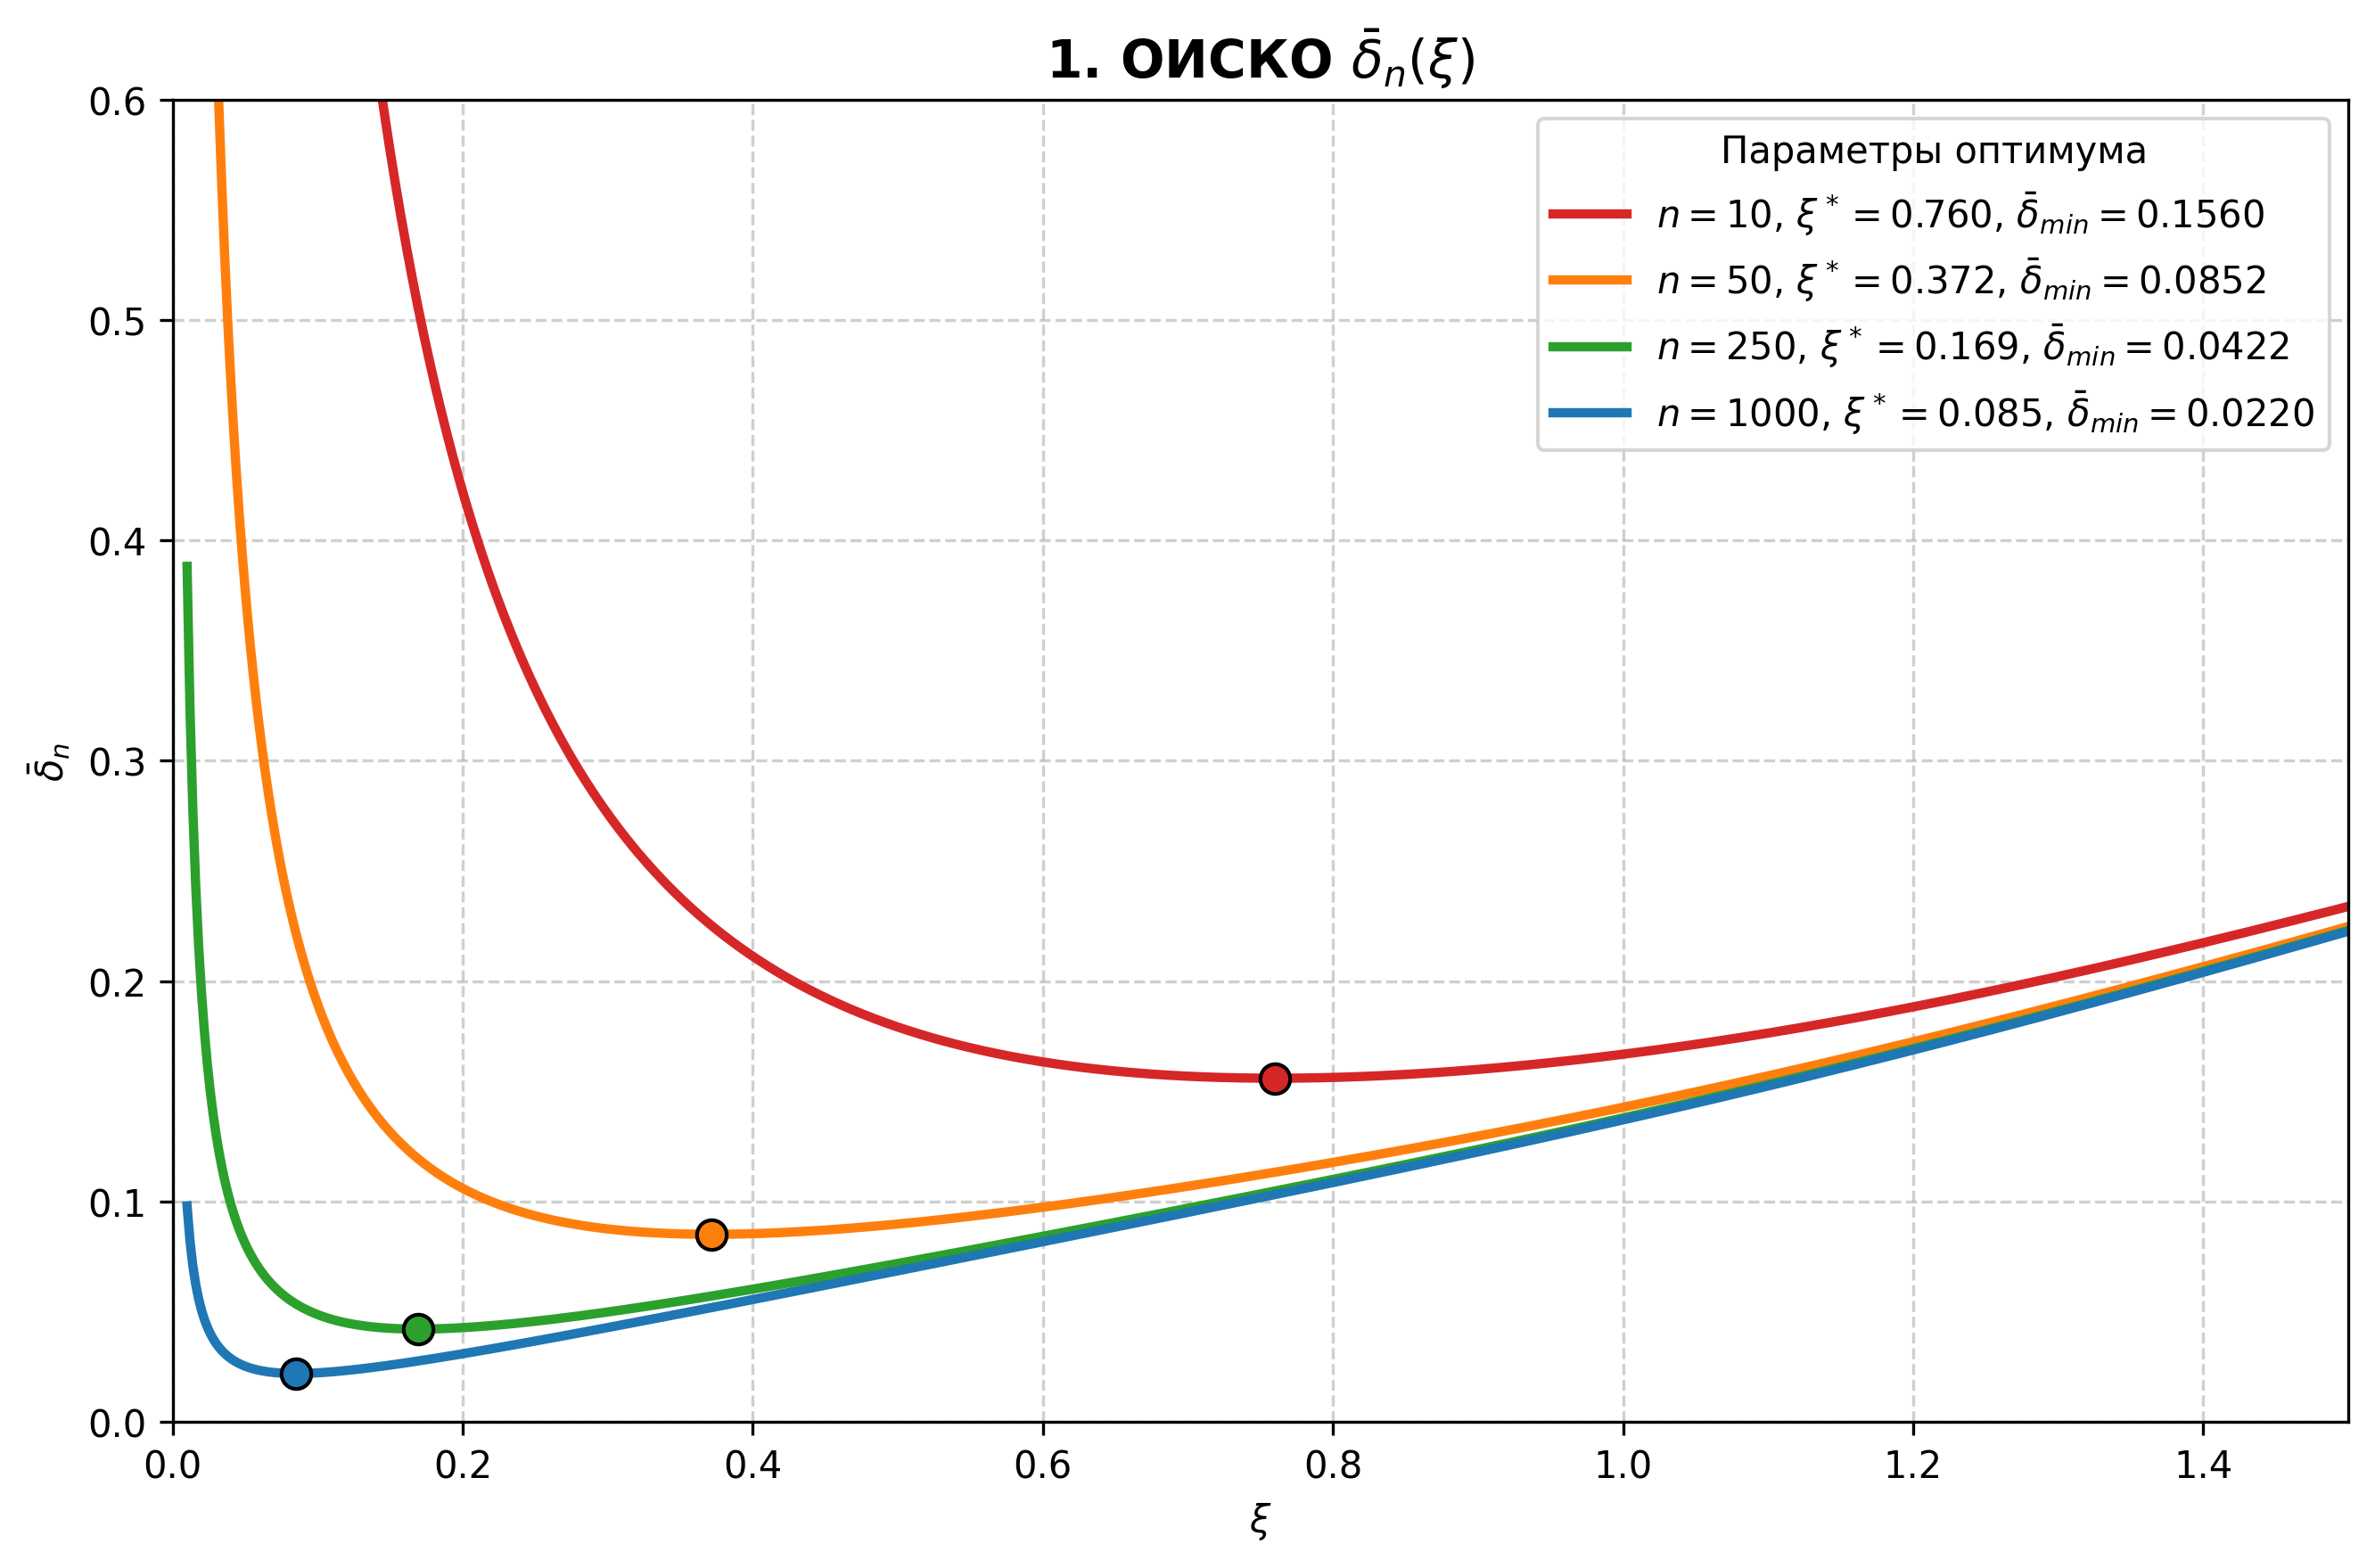
\includegraphics[width=0.85\textwidth]{figures/f1.png}
    \caption{ОИСКО \(\bar{\delta}_n(\xi)\) для разных объёмов выборки \(n = 10, 50, 250, 1000\)}
    \label{fig:delta_xi}
\end{figure}

\subsection*{График 2. Зависимость оптимального параметра \(\xi_{opt}\) от объёма выборки \(n\)}

\begin{figure}[ht!]
    \centering
    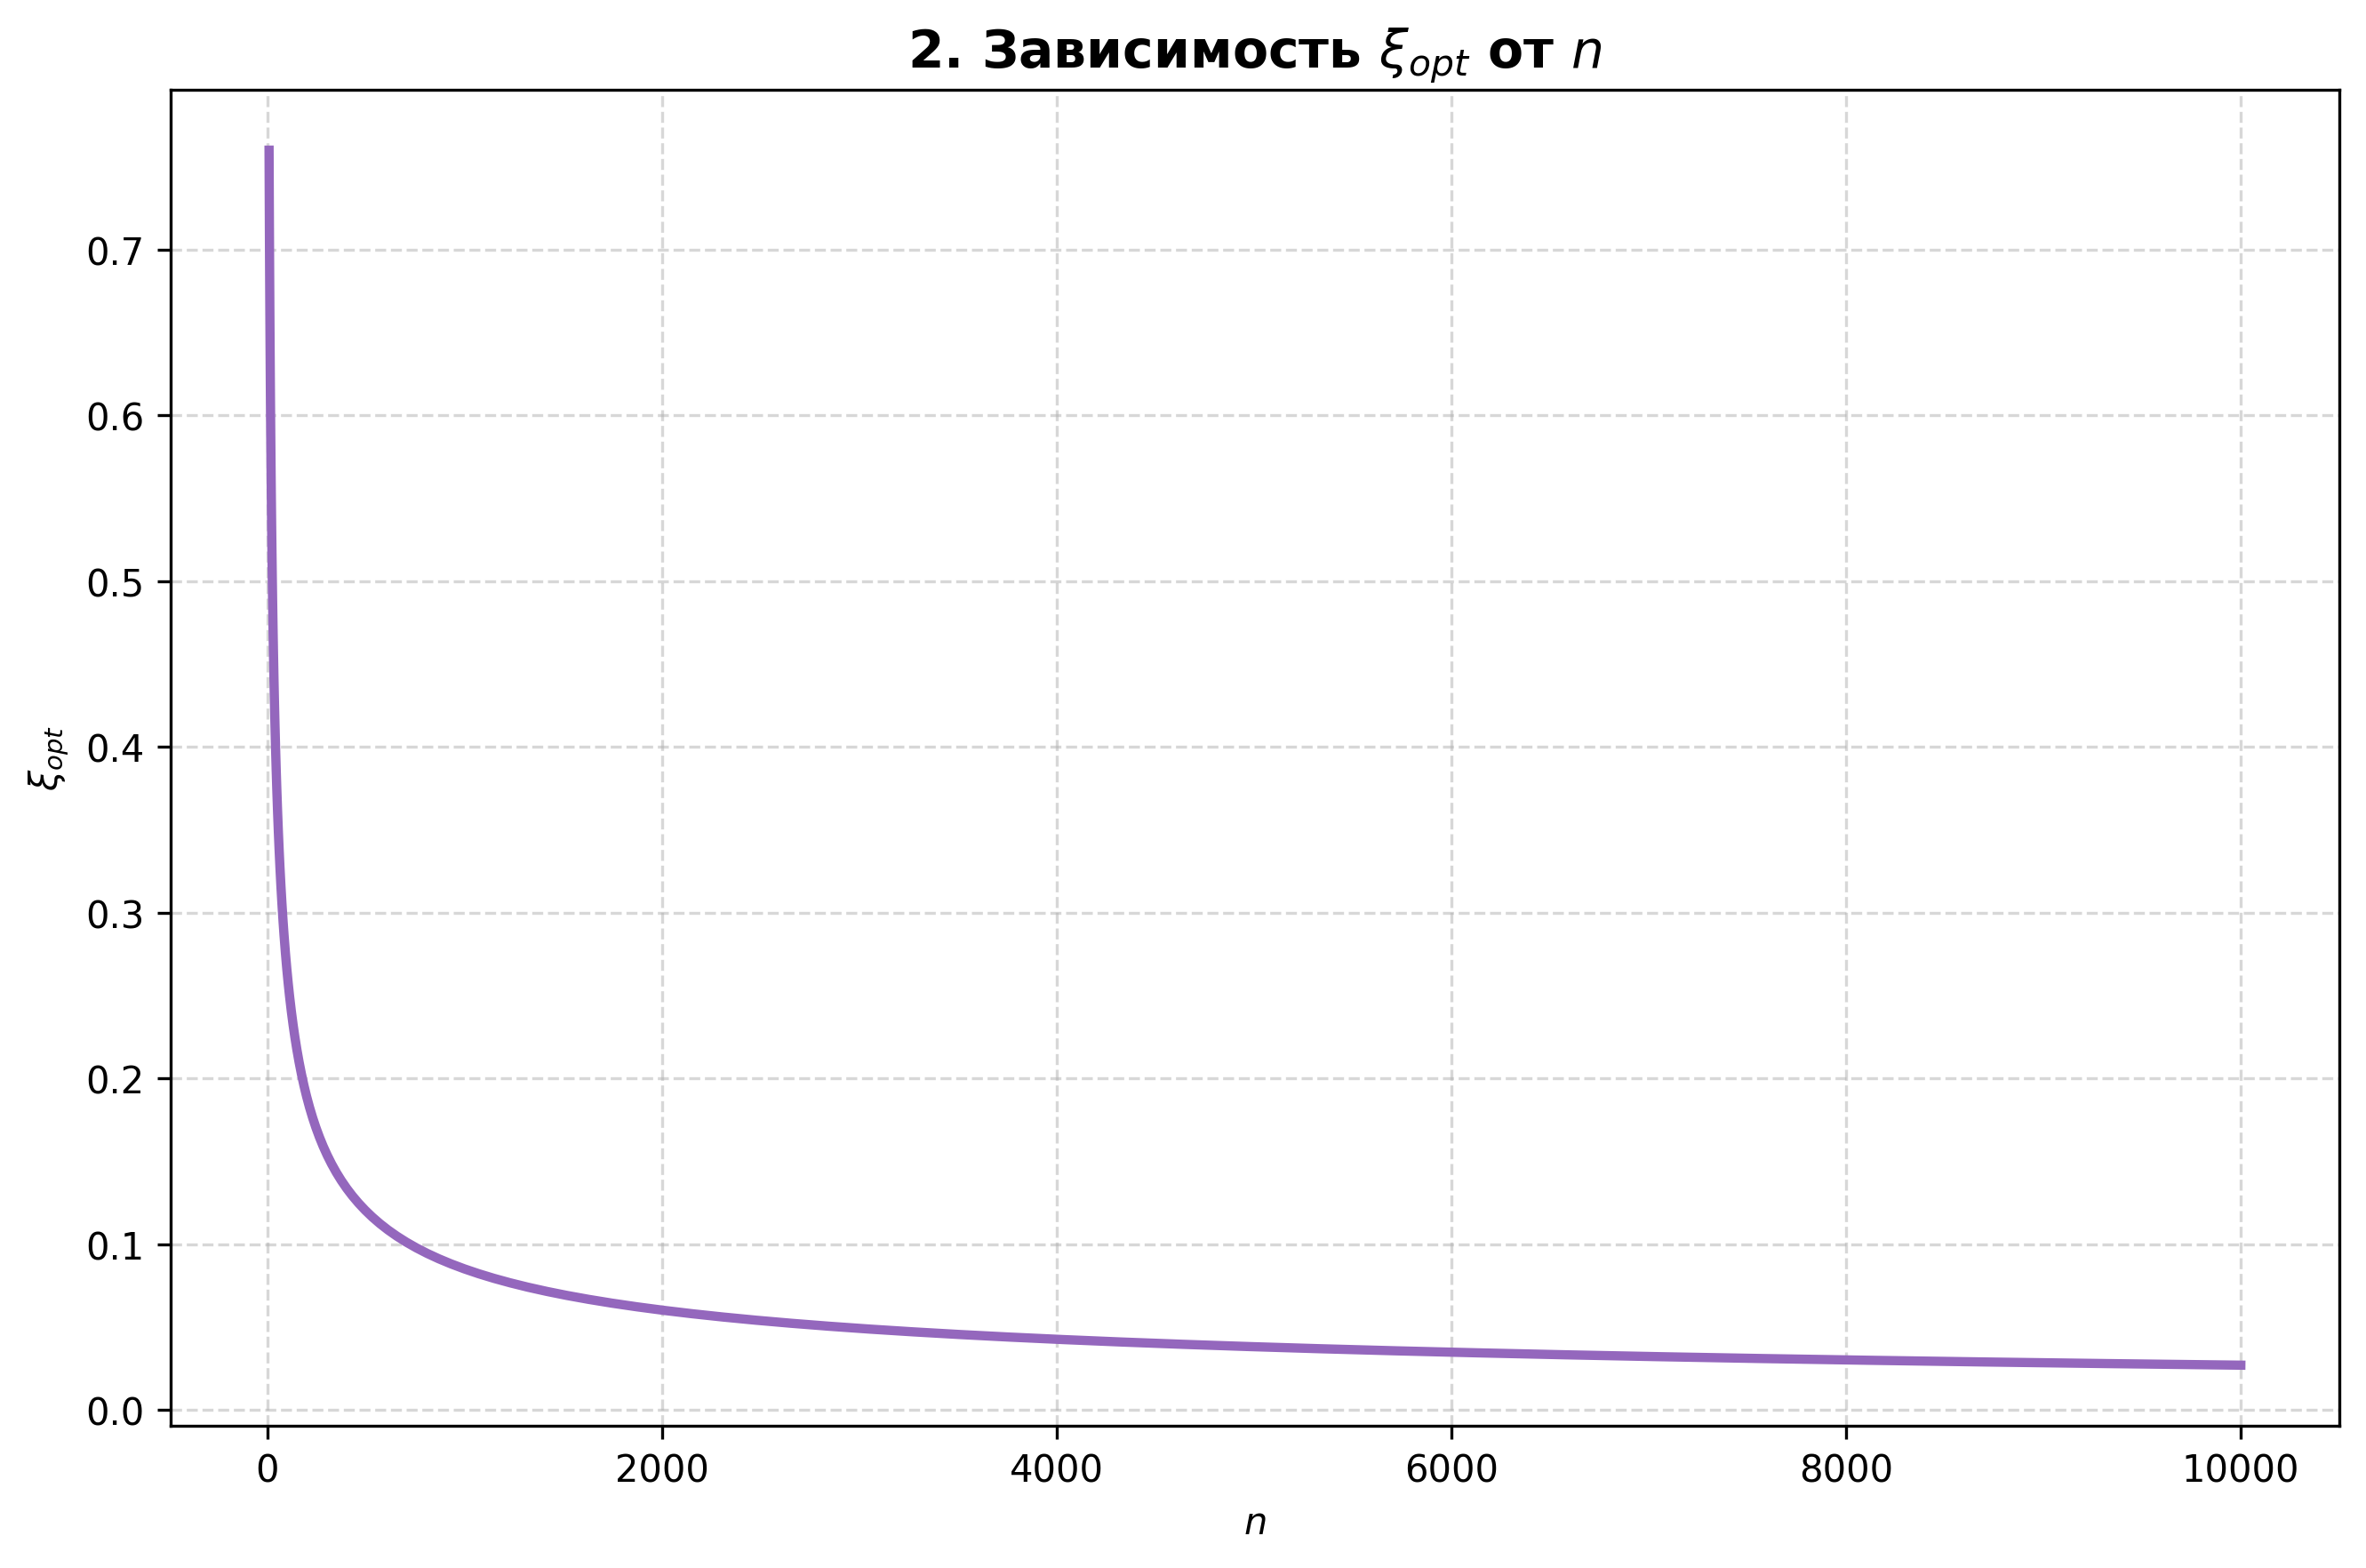
\includegraphics[width=0.85\textwidth]{figures/f2.png}
    \caption{Зависимость оптимального параметра сглаживания \(\xi_{opt}\) от объёма выборки \(n\)}
    \label{fig:xi_opt}
\end{figure}

\newpage
\subsection*{График 3. Зависимость нижней границы погрешности \(\bar{\delta}_{n,\min}\) от объёма выборки \(n\)}

\begin{figure}[ht!]
    \centering
    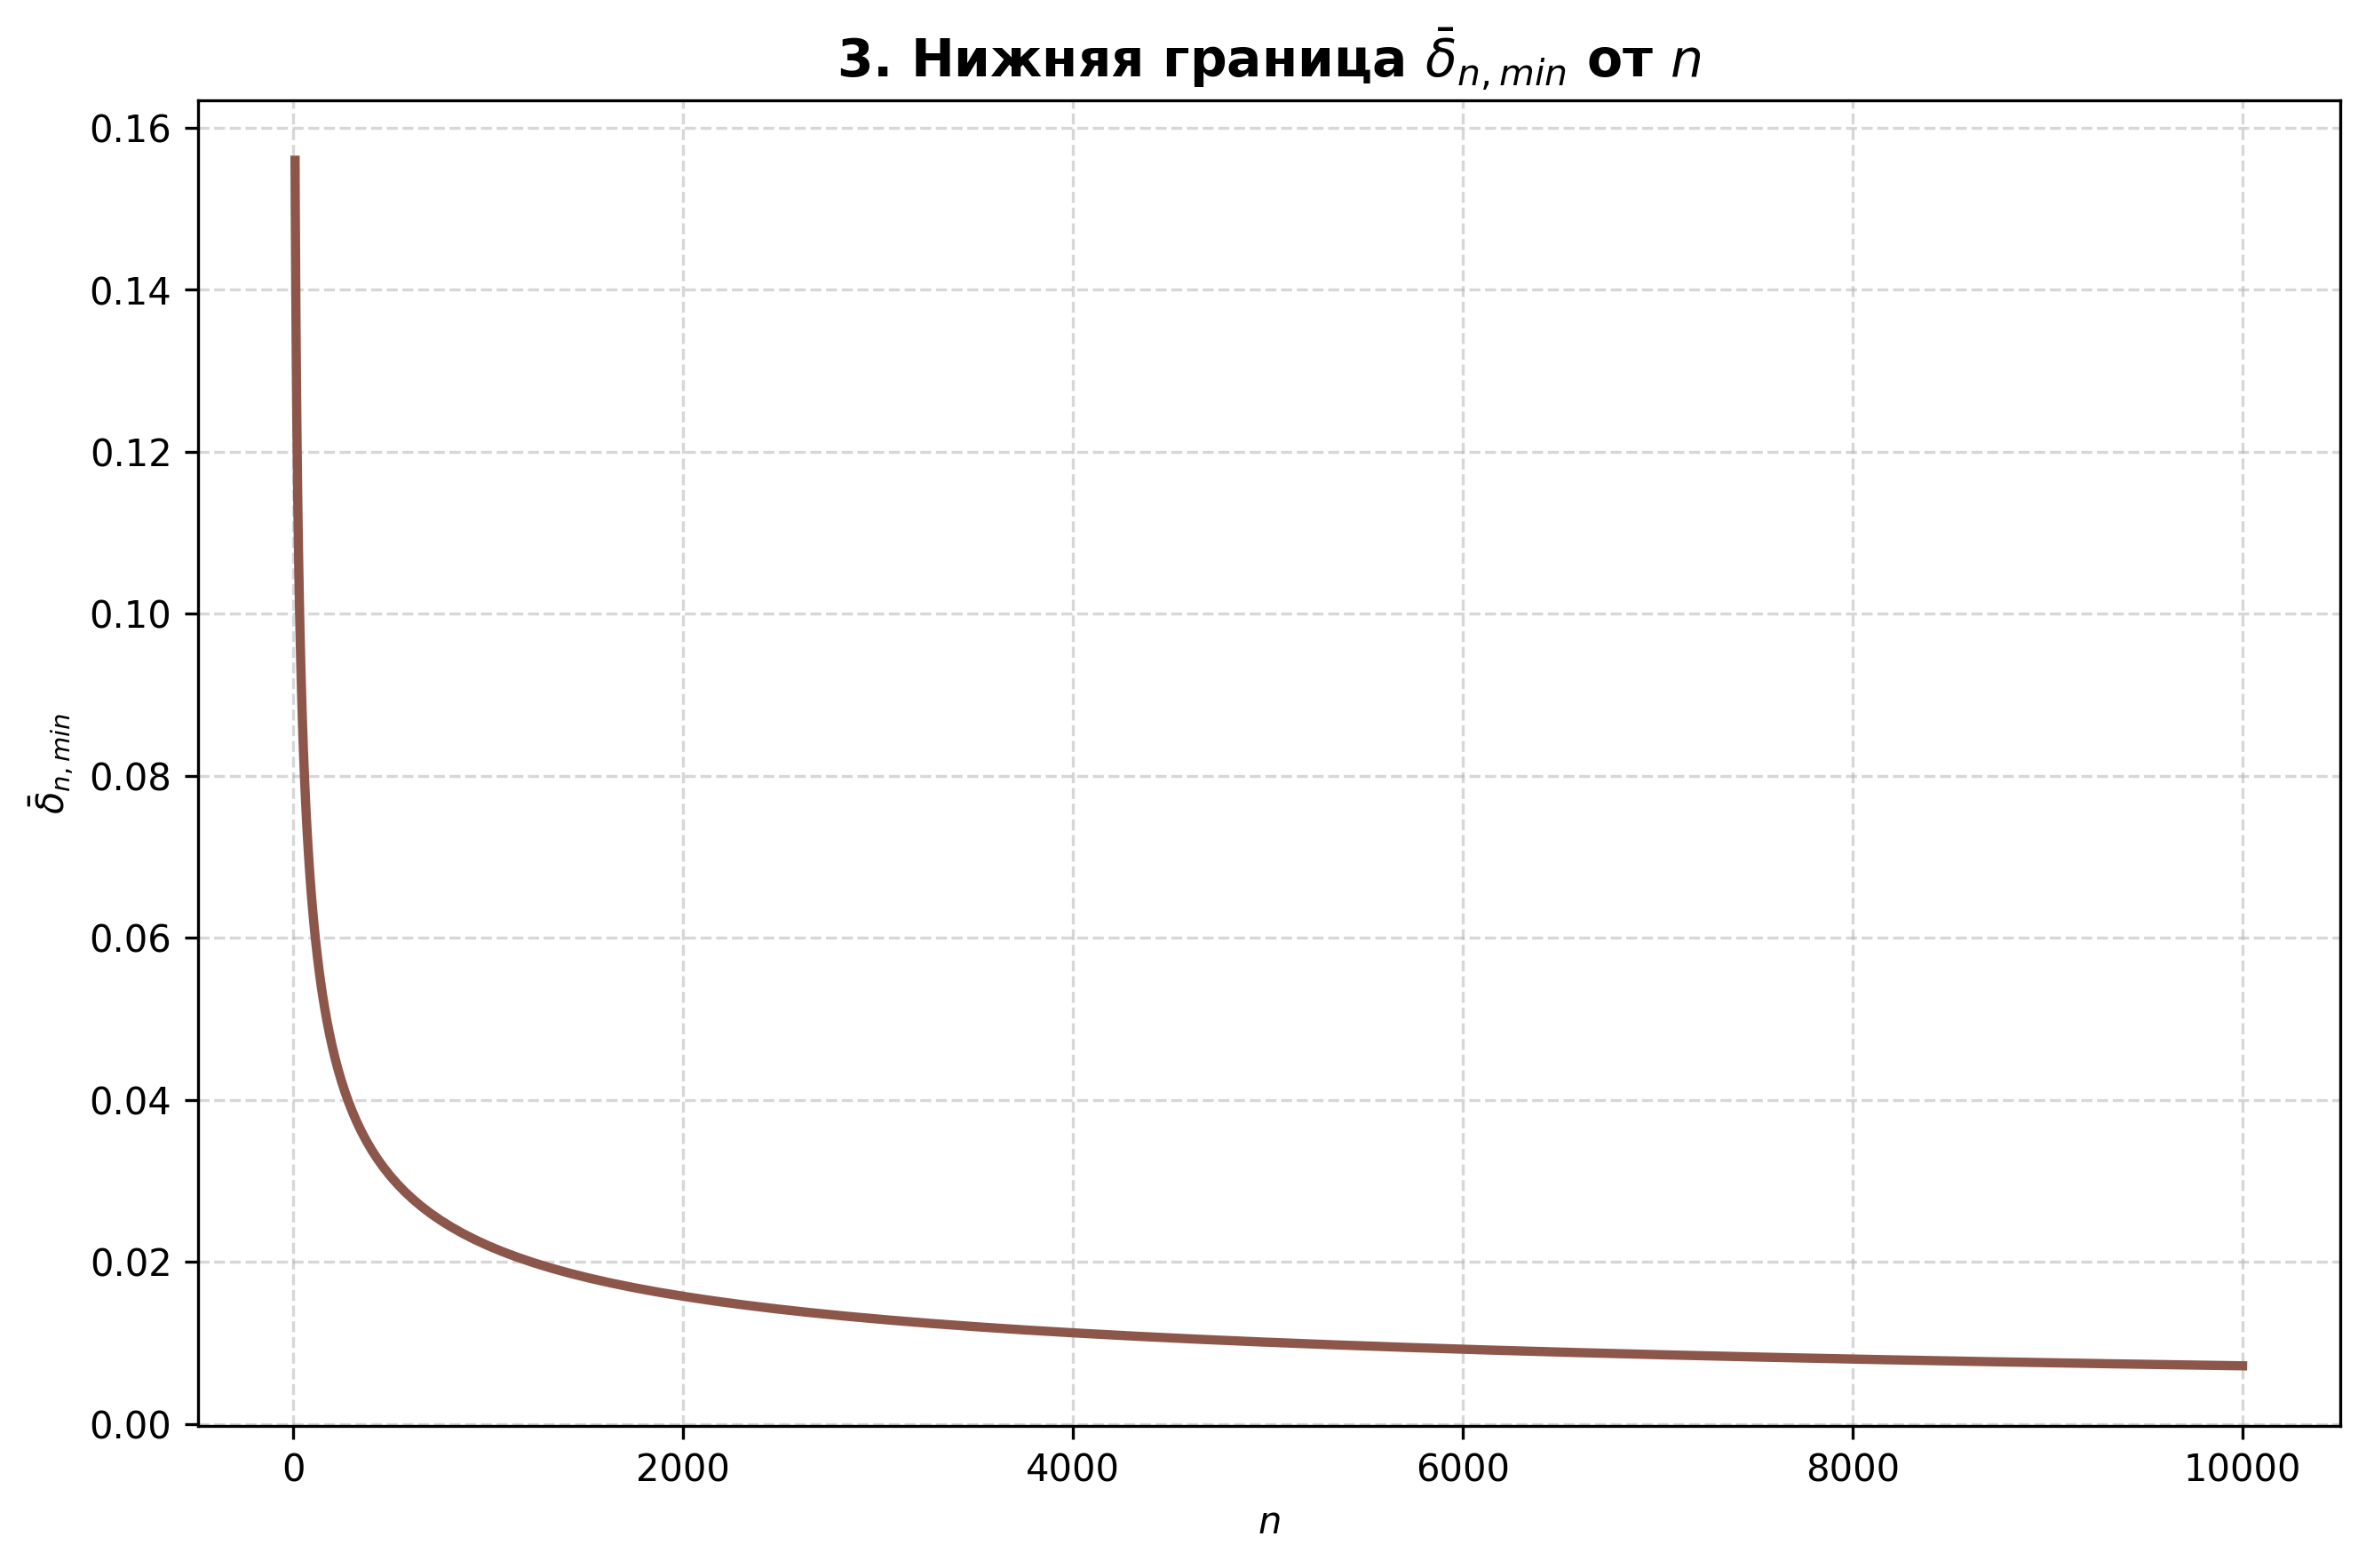
\includegraphics[width=0.85\textwidth]{figures/f3.png}
    \caption{Зависимость минимального значения ОИСКО \(\bar{\delta}_{n,\min}\) от объёма выборки \(n\)}
    \label{fig:delta_min}
\end{figure}

\subsection*{График 4. Эффективность ядерной оценки \(e_n(\xi)\)}

\begin{figure}[ht!]
    \centering
    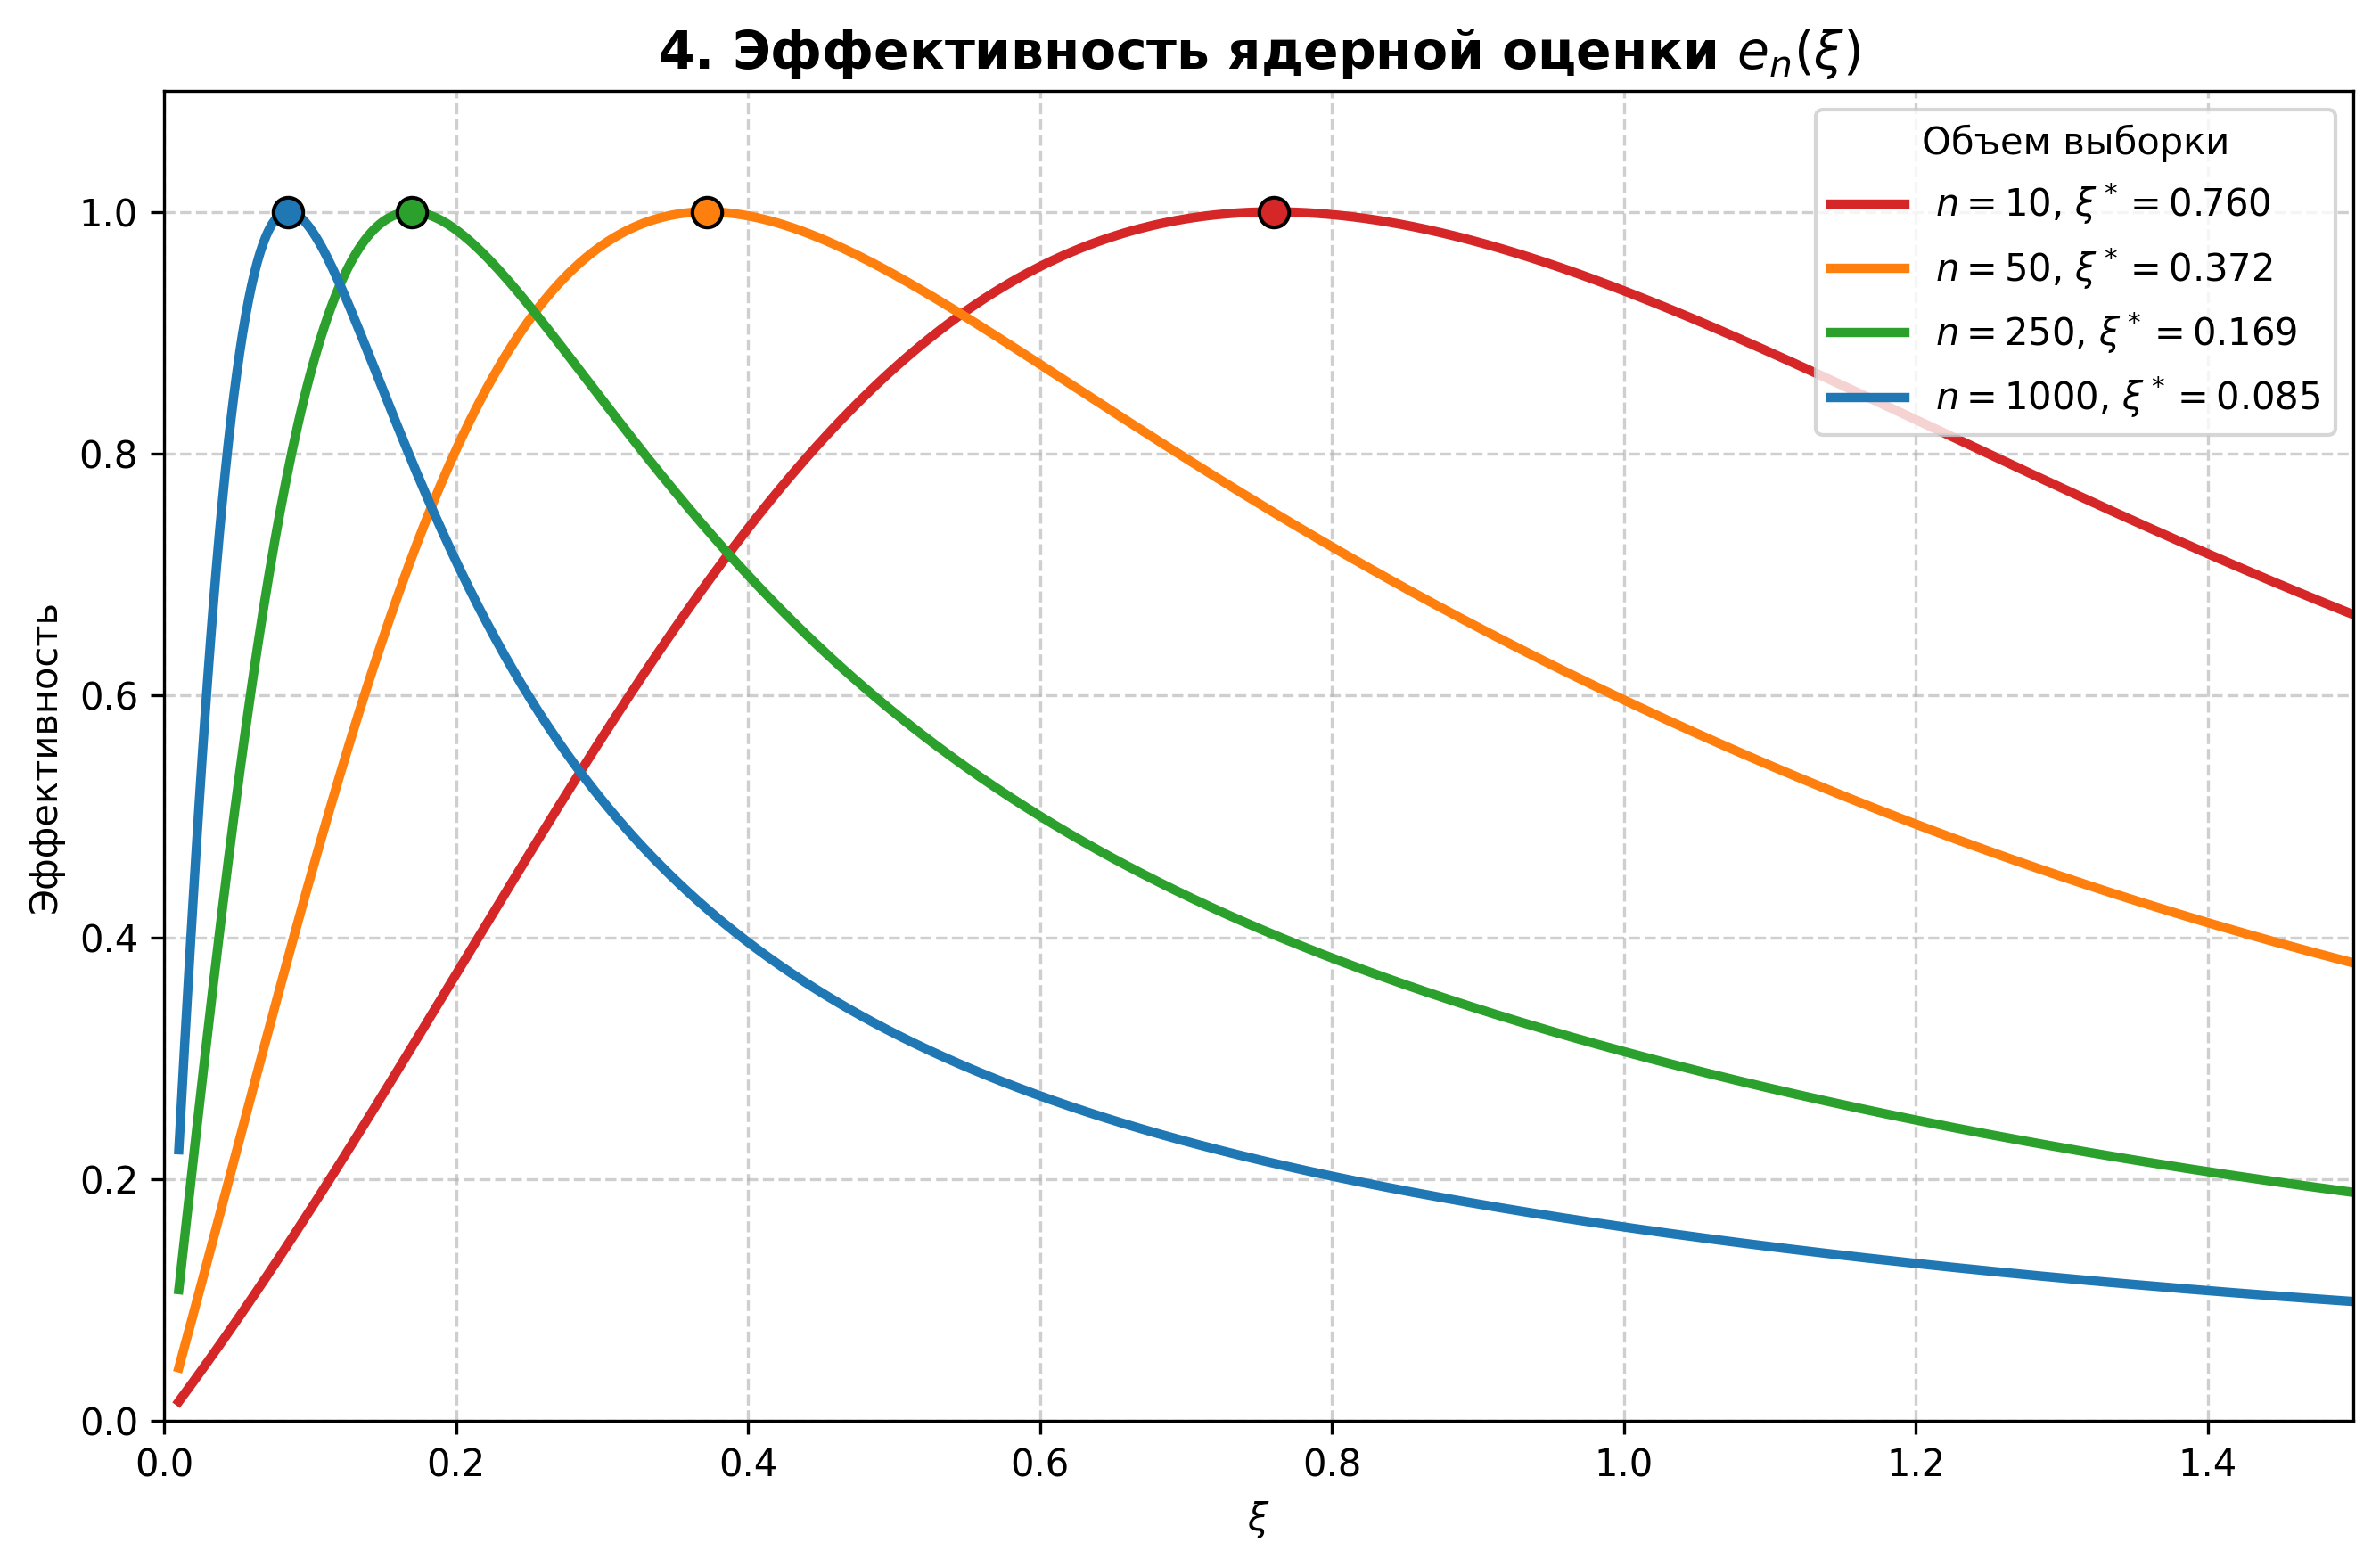
\includegraphics[width=0.85\textwidth]{figures/f4.png}
    \caption{Эффективность ядерной оценки \(e_n(\xi) = \bar{\delta}_{n,\min} / \bar{\delta}_n(\xi)\) для разных объёмов выборки}
    \label{fig:efficiency}
\end{figure}



\end{document}